Les séries v4 se jouent dans les conditions de calibration de \code{UCI\_Elo} : 60~s~+~0{,}6~s,
Stockfish~16 sur 1 thread avec Hash 16~Mo (préréglage \code{uci-elo}). Toutes ont tourné sur la
même RTX PRO 6000. Le tableau donne les médianes par partie : débit, profondeur moyenne de notre
moteur et profondeur de Stockfish.

\begin{table}[H]
\centering\scriptsize\begin{tabular}{lcccccccrrrr}
\toprule
série & 1320 & 1500 & 1700 & 1900 & 2200 & 2500 & max & total & nœuds/s & prof. & prof. SF\\
\midrule
v4-hybride-ucielo & 0/2 & 0/2 & -- & -- & -- & -- & -- & 0/4 & $1{,}2\cdot 10^{7}$ & 6{,}4 & 29\\
v4-plein-ucielo & 1{,}5/2 & 1/2 & 1{,}5/2 & 0{,}5/2 & 1/2 & 0/2 & 0/2 & 5{,}5/14 & $2{,}5\cdot 10^{8}$ & 4{,}8 & 32\\
v4-hybride-machine & -- & -- & -- & -- & -- & -- & 0/2 & 0/2 & $4{,}1\cdot 10^{7}$ & 6{,}9 & 65\\
v4b-hybride-ucielo-corrige & 2/2 & 1{,}5/2 & 1/2 & 1/2 & 1{,}5/2 & 0{,}5/2 & 0/2 & 7{,}5/14 & $1{,}9\cdot 10^{7}$ & 6{,}4 & 35\\
\bottomrule
\end{tabular}

\caption{Séries v4. \code{v4-hybride-ucielo} a été jouée avant le correctif de racine décrit
ci-dessous ; \code{v4b} est la même série après correctif. \code{v4-hybride-machine} oppose
l'hybride à Stockfish sur toute la machine (30 threads, Hash 8~Go).}
\end{table}

\begin{figure}[H]
\centering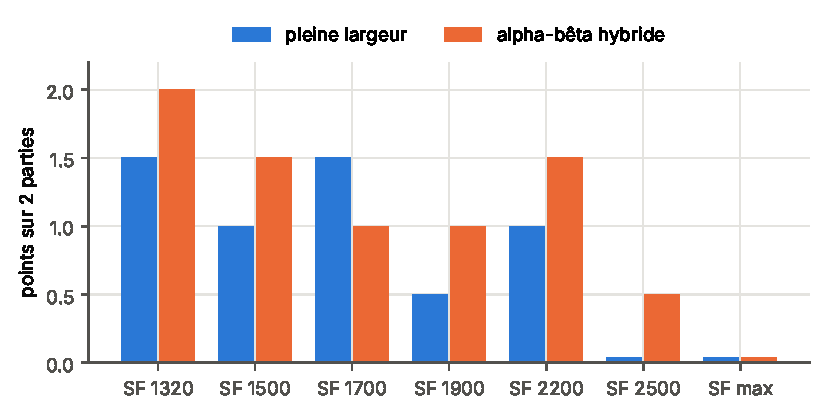
\includegraphics[width=0.85\linewidth]{scores_ucielo.pdf}
\caption{Conditions de calibration (60~s~+~0{,}6~s) : alpha-bêta hybride corrigé contre pleine
largeur, deux parties par niveau.}
\end{figure}

\paragraph{Un bug trouvé par les matchs.} La première série hybride a perdu ses quatre parties,
dont des mats en 22 et 25 demi-coups, alors qu'elle cherchait plus profond (6{,}4 en moyenne
contre 4{,}8). La cause était à la racine. Les coups autres que le premier sont cherchés avec la
fenêtre $(-\infty,-s_0)$, et leur score fail-soft n'est alors qu'une borne haute, souvent égale à
$s_0$. Sur une égalité, \code{argmax} renvoyait le premier indice du tableau, parfois un coup
réfuté. Le test d'équivalence ne comparait que le score, pas le coup joué : il ne pouvait pas le
voir. Le correctif place ces bornes strictement sous $s_0$. Un nouveau test exige que la valeur
exacte du coup joué égale la valeur minimax ; il échouait avant le correctif.

\paragraph{Résultats après correctif.}
\begin{itemize}
\item L'alpha-bêta hybride marque \textbf{7{,}5/14}, contre 5{,}5/14 pour la pleine largeur. C'est
le meilleur total de toutes les séries, avec 1{,}5/2 contre Stockfish 2200 et 0{,}5/2 contre 2500.
Il cherche à 6{,}4 demi-coups en médiane, contre 4{,}8, avec un débit 13 fois plus faible
($1{,}9\cdot10^7$ contre $2{,}5\cdot10^8$ nœuds/s).
\item Sur 14 parties par série, l'écart de 2 points ne départage rien statistiquement : l'erreur
type de l'écart entre deux séries vaut environ $\pm130$ Elo. Il va dans le sens prévu par l'avocat du diable, pour qui la
profondeur est le facteur limitant.
\item Face à Stockfish sur toute la machine, Stockfish calcule $2{,}8$ à $3{,}5\cdot10^7$ nœuds/s,
contre $3{,}6$ à $4{,}7\cdot10^7$ pour nous. L'avantage de débit brut tombe à environ 1{,}3, alors
qu'il était de 100 à 300 face à un seul thread. Stockfish voit 63 à 67 demi-coups, nous 7. Les deux
parties sont perdues.
\end{itemize}
